\documentclass[wide]{adonis}

\usepackage{graphicx}

\newpage
\chapter*{\centering Abstract}
\textit{\quad 
Write abstract of your theisis.
}



\begin{document}

\maketitle

\section{The CNN Architecture}

Convolutional Neural Networks (CNNs) are a special kind of multi-layer neural networks. Like almost every other neural networks they are trained with a version of the back-propagation algorithm. Where they differ is in the architecture. CNNs are designed to recognize visual patterns directly from pixel images with minimal preprocessing. They can recognize patterns with extreme variability (such as handwritten characters), and with robustness to distortions and simple geometric transformations. They are also known as shift invariant or space invariant artificial neural networks (SIANN), based on their shared-weights architecture and translation invariance characteristics.

\section{Principle}

CNNs for the most part, work by taking an input image and apply convolution operations over it with a kernel. The weights of the kernel is continuously updated over the period of training using back-propogation.

\begin{figure}
	\centering
	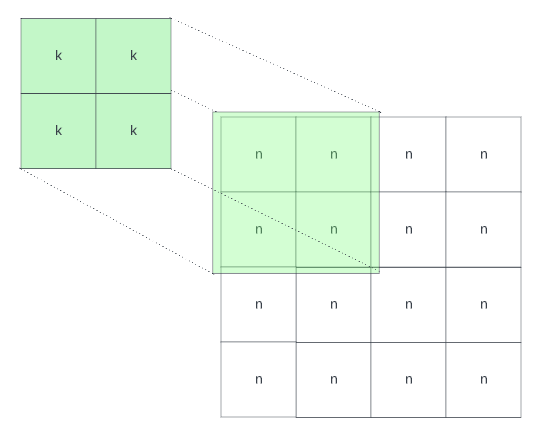
\includegraphics[width=0.5\textwidth]{images/convolution.png}
	\caption{Convolution operation}
	\label{convolution}
\end{figure}

Figure \ref{convolution} shows the convolution operation. The kernel is a matrix of weights which is applied over the input image. The kernel is slided over the image and the dot product of the kernel and the image is taken. The result of the dot product is stored in the output matrix. The kernel is slided over the image by a stride. The stride is the number of pixels by which the kernel is slided over the image. The kernel is slided over the image in both the horizontal and vertical direction. The output matrix is called the feature map. The feature map is smaller in size than the input image.

\section{PEMAN for CNN}

The PEMAN architecture can largely be used as-is for the CNN neural networks. This can be done by visualizing the CNN network in a different manner.

From the figure \ref{convolution}, we can see that the kernel values are being multiplied to the image pixel values and the output is being summed to give the output value for the feature map. This can be simplified as multiplication of weights to inputs and accumulating it to get the input. Going by this analogy, we can easily see that each convolution operation applied to the image with a kernel is a neuron. The output of each of the neuron contributes to the feature map.

By using this train of thought, we can also safely assume that PEMAN can be used for CNN architecture. The only difference is that the PEMAN architecture will not be emulating the convolution operation directly but rather, will be executing each operation inside.

The CNN process, through the previous analogy, can be distilled down to essentially a different kind of feedforward multi-layered neural network. Thus the weight updation process itself does not change except for the fact that the weights are updated for each neuron inside the convolution operation.

A CNN model is being depicted as a feedforward artifical neural network in Figure \ref{cnn_as_ann}

\begin{figure}
	\centering
	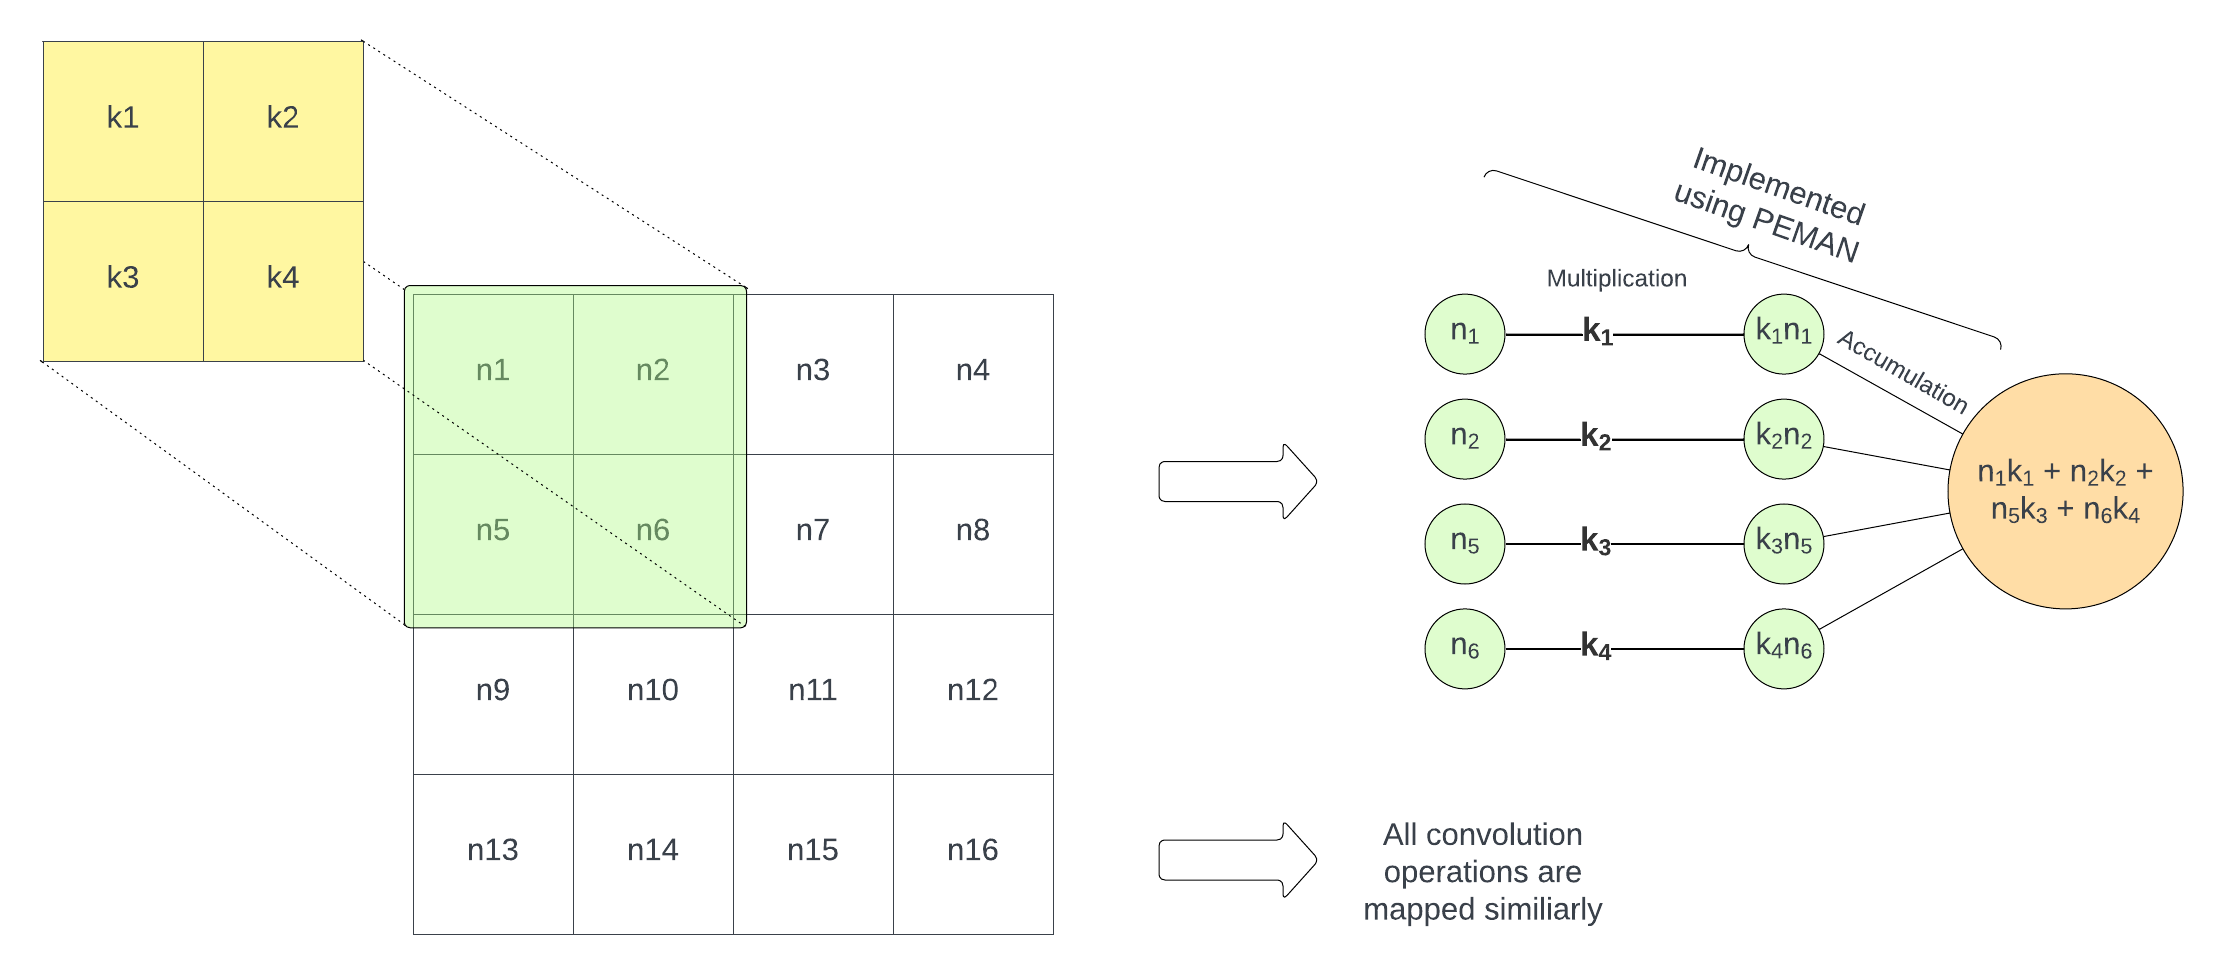
\includegraphics[width=\textwidth]{images/cnn_as_ann3.png}
	\caption{Realization of CNN as a more extensive ANN structure}
	\label{cnn_as_ann}
\end{figure}

The process that is being depicted in the image is as follows:

\begin{list}{•}{}
	\item The kernel is fit at the required position based on stride
	\item Each weight in the kernel needs to be multiplied with a image pixel.
	\item PEMAN structure scans the corresponding patch in the image and takes it as inputs and takes in the kernel as weights
	\item Each of these multiplications are done by a PEMAN neuron.
	\item After each multiplication, the results are accumulated together until the entire kernel is traversed.
	\item The output pixel value is attaine, which is passed onto next layer
	\item The capacitor is cleared and the kernel is moved again as per stride to repeast the processed again.
\end{list}

From the steps outlined below, we can conclude that the timing diagram for such a structure can be schematically represented as in Figure \ref{cnn_timing_diagram}

\begin{figure}
	\centering
	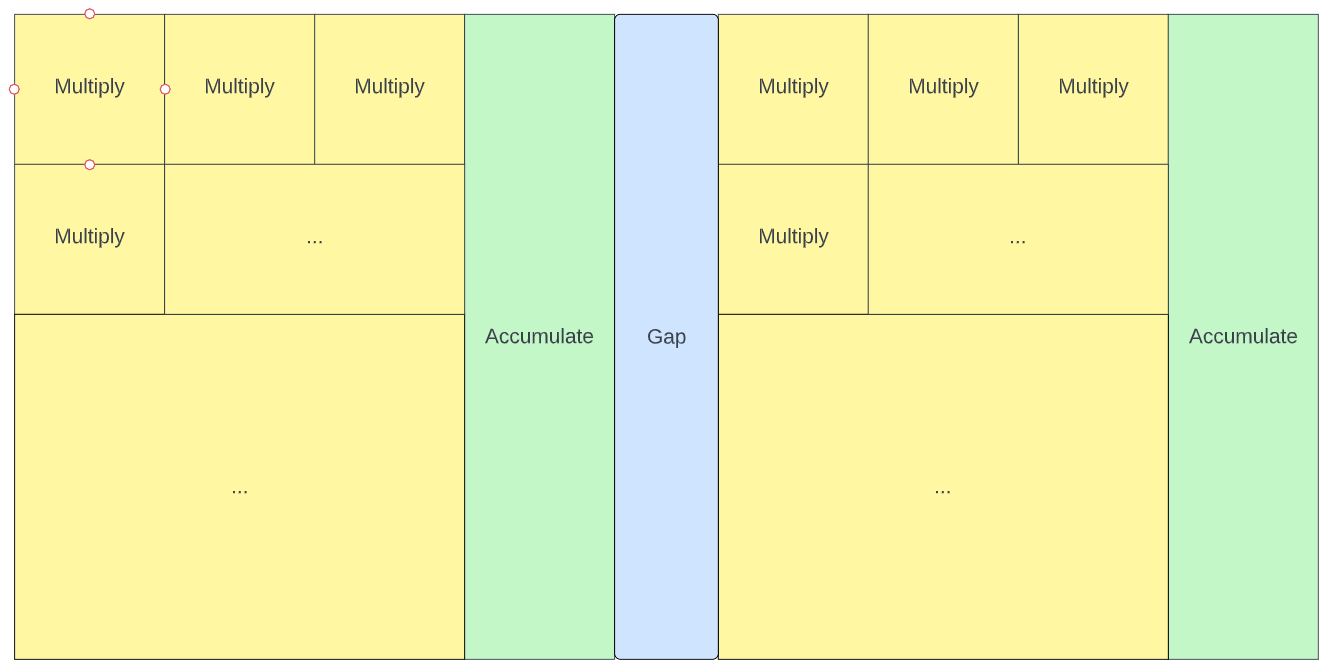
\includegraphics[width=\textwidth]{images/convTiming.png}
	\caption{Timing diagram for CNN}
	\label{cnn_timing_diagram}
\end{figure}

Let us assume the amount of time the PEMAN structure takes to do one multiplication operation is $T_{MUL}$, and the time it takes to ensure its ready for the next cycle is $T_S$.

Now, taking an image of $N\times N$ with a kernel size of $k \times k$, we study the total time it takes to process the entire image using this process.

The output image will be of size $(N - k + 1) \times (N - k + 1)$. Therefore, the total number of multiplication operations to be done will be

\begin{equation}
	\label{eqn:total_mul_ops}
	\begin{split}
		&\text{Total number of multiplication operations} \\
		&= \text{Number of pixels in output image} \times \text{Number of pixels in kernel} \\
		&= (N - k + 1)^2 \times k
	\end{split}
\end{equation}

But after each time an kernel is over, the PEMAN structure will take time to reset for the next cycle which needs to be acocunted for. Therefore, the total time taken to process the entire image will be

\begin{equation}
	\label{eqn:total_time}
	\begin{split}
		&T_{total} \\
		&= \text{Time taken for one kernel scanning} \times \text{Number of pixels in image} \\
		&= (T_{MUL} \times k + T_S) \times (N - k + 1)^2
	\end{split}
\end{equation}

Therefore, for a model containing multiple layers, either convolution or linear layers, the total time taken for one pass is

\begin{equation}
	\label{eqn:total_time_model}
	\begin{split}
		&T_{total} \\
		&= \text{Time taken for one kernel scanning} \times \text{Number of pixels in image} \\
		&= \sum_{n} (T_{MUL} \times k + T_S) \times (N - k + 1)^2
	\end{split}
\end{equation}

where n is the number of layers. For linear layers, the same formula os applicable but the kernel size of replace with 1.

This is the total time taken by one single PEMAN structure to emulate the convolution of a $k \times k$ kernel over an $N  \times N$ image once. In an CNN model, there might me multiple channels per layer, multiple images per batch and multiple convolution layers too, all of which needs to be taken into consideration, as per the model requirement.

Thus we can say that CNN can be emulated by the PEMAN structure when visualized as a modified form of Multi-Layered Perceptron. This can further be studied by looking into a practical exampke such as the MNIST dataset. The next chapter creates a CNN based deep learning model and implements it while simulating the PEMAN architecture to study the accuracy of the model.

\end{document}